\chapter{Systemarkitektur (David, Kasper og Kristian S.)}

\section{Version}
\begin{table}[h]
	\centering
	\begin{tabularx}{\textwidth - 2cm}{|l|l|l|X|}
	\hline
	Dato	& Version	& Initialer & Ændring	\\ \hline
	29. marts & 1 & KS & Første udkast. \\ \hline 
	\end{tabularx}
\end{table}

\section{Indledning}

\section{Udvidet Applikationsmodel}

\subsection{Sekvensdiagrammer}

\subsection{Usecase 1: Start}

\begin{figure}[!h]
\centering 
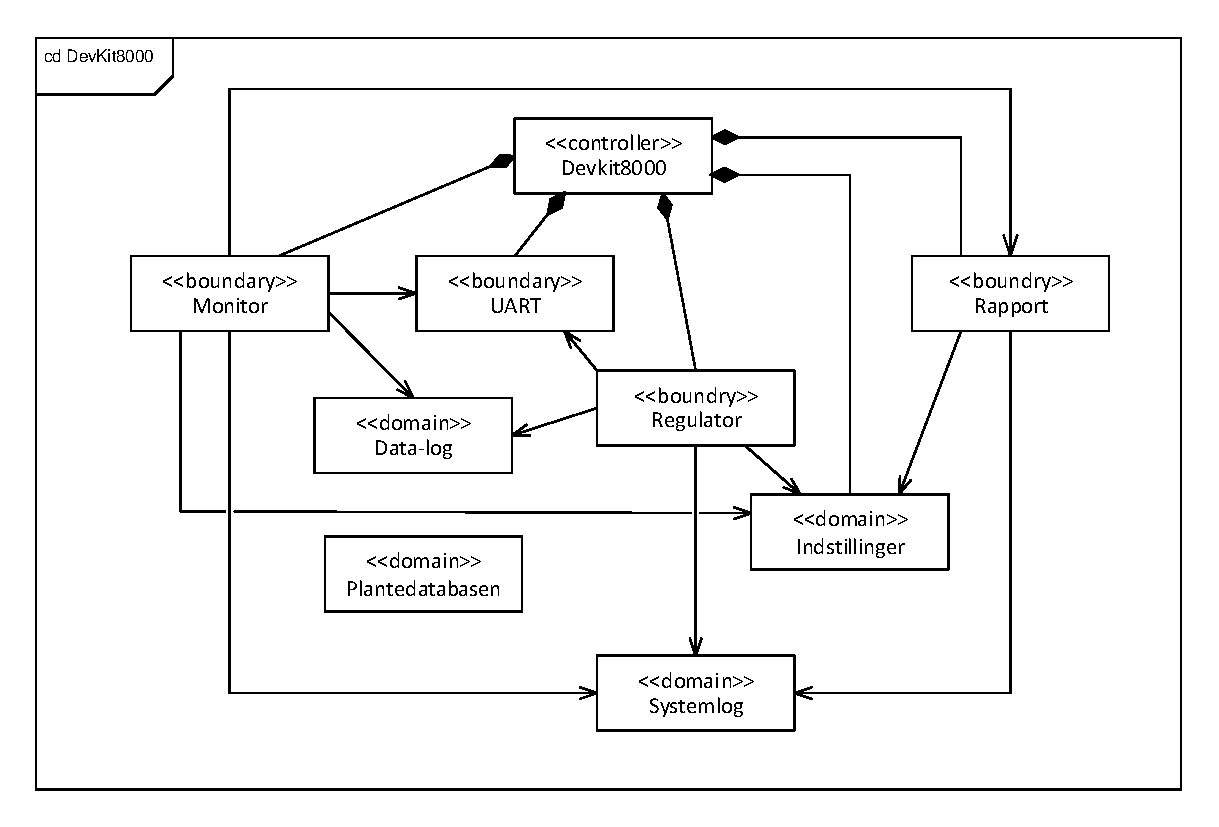
\includegraphics[scale=0.8] {../fig/UML_autogreen.pdf}
\caption{Application model for AutoGreen}
\label{fig:UML}
\end{figure}

\section{Klassebeskrivelser}

\subsection{Monitor}

%setTime
\begin{table}[h] 
\begin{tabularx}{\textwidth}{p{0.6 cm} l X} %\hline
\multicolumn{3}{l}{\textbf{setTime}}\\
& Operation: & %Skriv tekst herunder
\texttt{bool setTime( int time ) }
\\ & Parametre: & %Skriv tekst herunder
Modtager tidspunktet for hvornår en aktion skal udføres i minutter fra kl \texttt{00:00}. Dvs hvis en aktion skal starte kl \texttt{15:30} skal værdien $15 \times 60 + 30 = 930$ indsættes.
\\ & Returværdi: & %Skriv tekst herunder
Returnerer \texttt{TRUE}, hvis input var gyldigt og \texttt{FALSE} hvis ikke.
\\ & Beskrivelse: & %Skriv tekst herunder
Set-metode til at vælge hvilket tidspunkt, den givne aktion skal udføres. Metoden ændrer udelukkende på variablen \texttt{minutes}.
\\ \end{tabularx}
\end{table}


\section{GUIbeskrivelse}

\section{Trådhåndtering}

\section{Datastrukturdesign}